\documentclass[aspectratio=169,xcolor=table]{beamer}
\usetheme{Madrid}
\usecolortheme{default}

% Packages
\usepackage{lmodern}
\usepackage{graphicx}
\usepackage{booktabs}
\usepackage{tikz}
\usepackage{hyperref}
\usepackage{amssymb}
\usetikzlibrary{shapes,arrows,positioning}

% Graphics path
\graphicspath{{./}{./figures/}}

% Custom colors
\definecolor{mabscessus}{RGB}{0,191,255}
\definecolor{mtb}{RGB}{255,165,0}
\definecolor{dnacolor}{RGB}{0,0,139}
\definecolor{rosetta}{RGB}{139,69,19}

% Title information
\title[RosettaCM Homology Modeling]{RosettaCM Comparative Modeling:\\
Homology Modeling of DNA Gyrase}
\subtitle{Hybridize Protocol, FastRelax \& Model Validation}
\author{Roy Ahmed}
\institute{Computational Structural Biology}
\date{February 18, 2026}

\begin{document}

%=========================================
% TITLE SLIDE
%=========================================
\begin{frame}
\titlepage
\end{frame}

%=========================================
% OUTLINE
%=========================================
\begin{frame}{Outline}
\tableofcontents
\end{frame}

%=========================================
\section{Introduction}
%=========================================
\begin{frame}{The Modeling Problem}

\begin{columns}
\column{0.55\textwidth}
\textbf{Challenge: No Experimental Structure}
\begin{itemize}
    \item Target: \textit{M. abscessus} DNA gyrase
    \item No X-ray or cryo-EM structure available
    \item Homologous template exists (PDB 5BS8)
    \item Sequence identity: $\sim$70\%
    \item Large multi-subunit complex (GyrA$_2$GyrB$_2$)
\end{itemize}

\vspace{0.3cm}

\textbf{Modeling Requirements}
\begin{itemize}
    \item Build $>$3,000 residue tetramer
    \item Model loop regions de novo
    \item Preserve protein-DNA interface
    \item Energy minimize final structure
\end{itemize}

\column{0.45\textwidth}
\textbf{Why RosettaCM?}
\begin{itemize}
    \item \textbf{Hybridize protocol}: Multi-template threading
    \item \textbf{Fragment assembly}: Better loop modeling
    \item \textbf{Physics-based scoring}: Rosetta energy function
    \item \textbf{Full-atom refinement}: All-atom minimization
    \item \textbf{Validated}: Top performer in CASP
\end{itemize}

\vspace{0.3cm}

\begin{block}{Solution}
RosettaCM comparative modeling with FastRelax refinement
\end{block}
\end{columns}

\end{frame}

%=========================================
\section{How We Built the Model}
%=========================================
\begin{frame}{What is Homology Modeling?}

\textbf{Building a 3D structure when no experimental data exists}

\vspace{0.3cm}

\begin{columns}
\column{0.5\textwidth}
\textbf{The Basic Idea}
\begin{itemize}\setlength{\itemsep}{0pt}
    \item Proteins with similar sequences have similar shapes
    \item If we know a related protein's shape, use it as a ``blueprint''
\end{itemize}

\vspace{0.2cm}

\textbf{Our Situation}
\begin{itemize}\setlength{\itemsep}{0pt}
    \item \textbf{Target}: \textit{M. abscessus} gyrase (unknown)
    \item \textbf{Template}: \textit{M. tuberculosis} gyrase (known)
    \item \textbf{Similarity}: $\sim$70-95\% identical
\end{itemize}

\column{0.5\textwidth}
\begin{center}
\textbf{The Modeling Analogy}

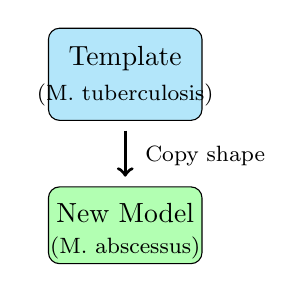
\begin{tikzpicture}[scale=0.65]
% Template
\draw[fill=cyan!30, rounded corners] (0,3) rectangle (3,4.8);
\node at (1.5, 4.2) {Template};
\node at (1.5, 3.5) {\footnotesize (M. tuberculosis)};

% Arrow
\draw[->, very thick] (1.5, 2.8) -- (1.5, 1.9);
\node[right] at (1.7, 2.3) {\footnotesize Copy shape};

% Model
\draw[fill=green!30, rounded corners] (0,0.2) rectangle (3,1.7);
\node at (1.5, 1.2) {New Model};
\node at (1.5, 0.5) {\footnotesize (M. abscessus)};
\end{tikzpicture}
\end{center}
\end{columns}

\begin{block}{Key Insight}
High sequence similarity (70\%+) means we can confidently predict the 3D structure
\end{block}

\end{frame}

%=========================================
\begin{frame}{The Modeling Process: Step by Step}

\begin{center}
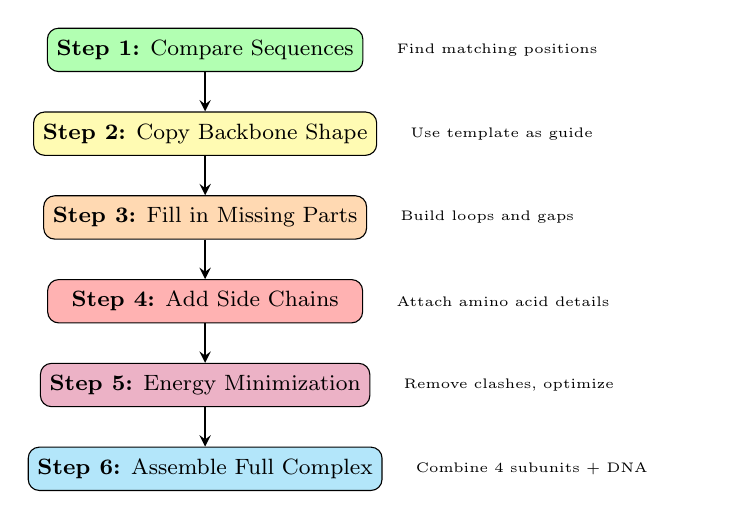
\begin{tikzpicture}[
    node distance=0.5cm,
    box/.style={rectangle, draw, rounded corners, minimum width=4cm, minimum height=0.55cm, align=center, font=\footnotesize},
    arrow/.style={->, thick, >=stealth}
]

\node[box, fill=green!30] (step1) {\textbf{Step 1:} Compare Sequences};
\node[box, fill=yellow!30, below=of step1] (step2) {\textbf{Step 2:} Copy Backbone Shape};
\node[box, fill=orange!30, below=of step2] (step3) {\textbf{Step 3:} Fill in Missing Parts};
\node[box, fill=red!30, below=of step3] (step4) {\textbf{Step 4:} Add Side Chains};
\node[box, fill=purple!30, below=of step4] (step5) {\textbf{Step 5:} Energy Minimization};
\node[box, fill=cyan!30, below=of step5] (step6) {\textbf{Step 6:} Assemble Full Complex};

\draw[arrow] (step1) -- (step2);
\draw[arrow] (step2) -- (step3);
\draw[arrow] (step3) -- (step4);
\draw[arrow] (step4) -- (step5);
\draw[arrow] (step5) -- (step6);

% Annotations
\node[right=0.3cm of step1, font=\tiny, text width=3.5cm] {Find matching positions};
\node[right=0.3cm of step2, font=\tiny, text width=3.5cm] {Use template as guide};
\node[right=0.3cm of step3, font=\tiny, text width=3.5cm] {Build loops and gaps};
\node[right=0.3cm of step4, font=\tiny, text width=3.5cm] {Attach amino acid details};
\node[right=0.3cm of step5, font=\tiny, text width=3.5cm] {Remove clashes, optimize};
\node[right=0.3cm of step6, font=\tiny, text width=3.5cm] {Combine 4 subunits + DNA};

\end{tikzpicture}
\end{center}

\end{frame}

%=========================================
\begin{frame}{Energy Scoring: Evaluating Model Quality}

\textbf{Rosetta's scoring function assigns an energy value to each structure}

\vspace{0.2cm}

\begin{columns}
\column{0.5\textwidth}
\textbf{The Algorithm Computes:}
\begin{itemize}\setlength{\itemsep}{2pt}
    \item \textbf{Van der Waals}: Steric clashes between atoms
    \item \textbf{Hydrogen bonds}: Stabilizing interactions
    \item \textbf{Solvation}: Hydrophobic/hydrophilic balance
    \item \textbf{Ramachandran}: Backbone $\phi$/$\psi$ angles
    \item \textbf{Electrostatics}: Charge-charge interactions
\end{itemize}

\column{0.5\textwidth}
\begin{center}
\textbf{Energy Minimization}
\vspace{0.2cm}

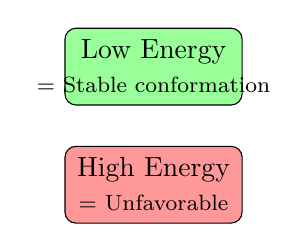
\begin{tikzpicture}[scale=0.75]
% Good structure
\draw[fill=green!40, rounded corners] (0,2) rectangle (3,3.3);
\node at (1.5, 2.9) {Low Energy};
\node at (1.5, 2.35) {\footnotesize = Stable conformation};

% Bad structure  
\draw[fill=red!40, rounded corners] (0,0) rectangle (3,1.3);
\node at (1.5, 0.9) {High Energy};
\node at (1.5, 0.35) {\footnotesize = Unfavorable};
\end{tikzpicture}
\end{center}

\begin{block}{Objective}
Minimize total energy to find the most thermodynamically favorable structure
\end{block}
\end{columns}

\end{frame}

%=========================================
\begin{frame}{Step 1: Comparing the Sequences}

\textbf{Finding which parts of the two proteins match up}

\vspace{0.3cm}

\begin{columns}
\column{0.55\textwidth}
\textbf{What is Sequence Alignment?}
\begin{itemize}
    \item Line up amino acids from both proteins
    \item Identify identical positions (conserved)
    \item Find gaps where one protein has extra/fewer parts
\end{itemize}

\vspace{0.2cm}

\textbf{Example:}
\begin{center}
\footnotesize
\texttt{M. tuberculosis: MSDLE\textcolor{red}{R}EITGPR...}\\
\texttt{M. abscessus:    MSDLE\textcolor{red}{R}EITGPR...}\\
\texttt{                 *****\textcolor{red}{*}******}
\end{center}
\footnotesize (* = identical positions)
\normalsize

\column{0.45\textwidth}
\textbf{Our Alignment Results}
\begin{table}
\centering
\footnotesize
\begin{tabular}{lcc}
\toprule
\textbf{Protein} & \textbf{Length} & \textbf{Identity} \\
\midrule
GyrA & 838 aa & $\sim$70\% \\
GyrB & 714 aa & $\sim$95\% \\
\bottomrule
\end{tabular}
\end{table}

\vspace{0.3cm}

\begin{alertblock}{High Similarity}
70-95\% identity means the proteins are very similar -- excellent for modeling
\end{alertblock}
\end{columns}

\end{frame}

%=========================================
\begin{frame}{Step 2: Using the Template as a Blueprint}

\textbf{The known structure guides our model construction}

\vspace{0.3cm}

\begin{columns}
\column{0.55\textwidth}
\textbf{What We Get From the Template}
\begin{itemize}
    \item \textbf{Overall shape}: How the protein folds
    \item \textbf{Subunit arrangement}: How the 4 pieces fit together
    \item \textbf{DNA position}: Where the DNA binds
    \item \textbf{Active site}: Location of drug binding pocket
\end{itemize}

\vspace{0.3cm}

\textbf{Template Details}
\begin{itemize}
    \item \textbf{Source}: PDB 5BS8 (\textit{M. tuberculosis})
    \item \textbf{Method}: X-ray crystallography
    \item \textbf{Resolution}: 2.5-3.0 \AA\ (good quality)
\end{itemize}

\column{0.45\textwidth}
\begin{center}
\textbf{Template Components}
\vspace{0.2cm}

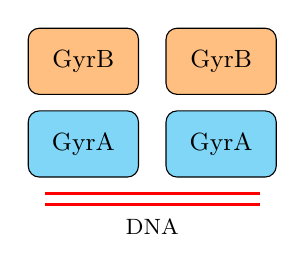
\begin{tikzpicture}[scale=0.7]
% GyrA
\draw[fill=cyan!50, rounded corners] (0,0) rectangle (2,1.2);
\node at (1, 0.6) {\small GyrA};
\draw[fill=cyan!50, rounded corners] (2.5,0) rectangle (4.5,1.2);
\node at (3.5, 0.6) {\small GyrA};

% GyrB
\draw[fill=orange!50, rounded corners] (0,1.5) rectangle (2,2.7);
\node at (1, 2.1) {\small GyrB};
\draw[fill=orange!50, rounded corners] (2.5,1.5) rectangle (4.5,2.7);
\node at (3.5, 2.1) {\small GyrB};

% DNA
\draw[very thick, red] (0.3,-0.3) -- (4.2,-0.3);
\draw[very thick, red] (0.3,-0.5) -- (4.2,-0.5);
\node at (2.25, -0.9) {\footnotesize DNA};
\end{tikzpicture}
\end{center}

\vspace{0.2cm}

\begin{block}{4 Protein Subunits + DNA}
Complete enzyme complex
\end{block}
\end{columns}

\end{frame}

%=========================================
\begin{frame}{Step 3: Building the Model (Rosetta's Algorithm)}

\begin{columns}
\column{0.5\textwidth}
\textbf{Stage 1: Centroid Mode}
\begin{itemize}\setlength{\itemsep}{0pt}
    \item Thread sequence onto template backbone
    \item Simplified side-chain representation
\end{itemize}

\textbf{Stage 2: Full-Atom Mode}
\begin{itemize}\setlength{\itemsep}{0pt}
    \item Rotamer optimization
    \item Position all heavy atoms
\end{itemize}

\textbf{Stage 3: Refinement}
\begin{itemize}\setlength{\itemsep}{0pt}
    \item Gradient descent minimization
    \item Optimize H-bond network
\end{itemize}

\column{0.5\textwidth}
\begin{center}
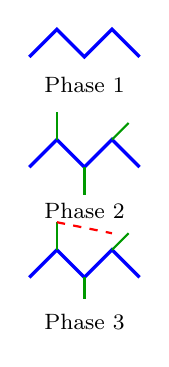
\begin{tikzpicture}[scale=0.7]
% Phase 1
\draw[very thick, blue] (0,4) -- (0.5,4.5) -- (1,4) -- (1.5,4.5) -- (2,4);
\node at (1, 3.5) {\footnotesize Phase 1};

% Phase 2
\draw[very thick, blue] (0,2) -- (0.5,2.5) -- (1,2) -- (1.5,2.5) -- (2,2);
\draw[thick, green!60!black] (0.5,2.5) -- (0.5,3);
\draw[thick, green!60!black] (1,2) -- (1,1.5);
\draw[thick, green!60!black] (1.5,2.5) -- (1.8,2.8);
\node at (1, 1.2) {\footnotesize Phase 2};

% Phase 3
\draw[very thick, blue] (0,0) -- (0.5,0.5) -- (1,0) -- (1.5,0.5) -- (2,0);
\draw[thick, green!60!black] (0.5,0.5) -- (0.5,1);
\draw[thick, green!60!black] (1,0) -- (1,-0.4);
\draw[thick, green!60!black] (1.5,0.5) -- (1.8,0.8);
\draw[dashed, red, thick] (0.5,1) -- (1.5,0.8);
\node at (1, -0.8) {\footnotesize Phase 3};
\end{tikzpicture}
\end{center}
\end{columns}

\begin{block}{Result}
Algorithm generates N conformations, selects lowest-energy model
\end{block}

\end{frame}

%=========================================
\begin{frame}{Step 4: Assembling the Complete Enzyme}

\textbf{DNA Gyrase is a team of 4 protein subunits}

\vspace{0.2cm}

\begin{columns}
\column{0.48\textwidth}
\textbf{The Assembly Process}
\begin{enumerate}\setlength{\itemsep}{0pt}
    \item Build individual subunit models
    \item Place them in correct positions
    \item Add the DNA strand
    \item Add magnesium ions
    \item Check everything fits
\end{enumerate}

\vspace{0.1cm}

\textbf{Why This Matters}
\begin{itemize}\setlength{\itemsep}{0pt}
    \item Drug binds at interface between subunits
    \item Need complete complex for docking
\end{itemize}

\column{0.52\textwidth}
\begin{center}
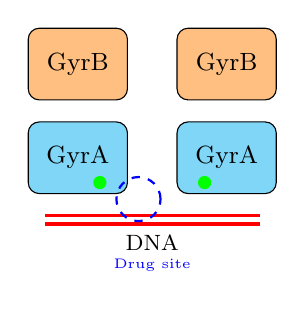
\begin{tikzpicture}[scale=0.7]
% GyrA subunits
\draw[fill=cyan!50, rounded corners] (0,0) rectangle (1.8,1.3);
\node at (0.9, 0.65) {\small GyrA};
\draw[fill=cyan!50, rounded corners] (2.7,0) rectangle (4.5,1.3);
\node at (3.6, 0.65) {\small GyrA};

% GyrB subunits
\draw[fill=orange!50, rounded corners] (0,1.7) rectangle (1.8,3);
\node at (0.9, 2.35) {\small GyrB};
\draw[fill=orange!50, rounded corners] (2.7,1.7) rectangle (4.5,3);
\node at (3.6, 2.35) {\small GyrB};

% DNA
\draw[very thick, red] (0.3,-0.4) -- (4.2,-0.4);
\draw[very thick, red] (0.3,-0.55) -- (4.2,-0.55);
\node at (2.25, -0.9) {\footnotesize DNA};

% Mg ions
\fill[green] (1.3, 0.2) circle (0.12);
\fill[green] (3.2, 0.2) circle (0.12);

% Drug binding site
\draw[dashed, blue, thick] (2,-0.1) circle (0.4);
\node[blue, font=\tiny] at (2.25, -1.3) {Drug site};
\end{tikzpicture}
\end{center}
\end{columns}

\end{frame}

%=========================================
\begin{frame}{Step 5: Final Polishing (Energy Minimization)}

\textbf{Making the model physically realistic}

\vspace{0.3cm}

\begin{columns}
\column{0.55\textwidth}
\textbf{What Happens in This Step}
\begin{itemize}
    \item \textbf{Remove atom clashes}: Atoms can't overlap in real life
    \item \textbf{Optimize bonds}: Adjust distances and angles
    \item \textbf{Find stable state}: Like a ball rolling to the bottom of a valley
\end{itemize}

\vspace{0.3cm}

\textbf{The Process}
\begin{enumerate}
    \item Start with loose constraints (allow big movements)
    \item Gradually tighten constraints
    \item Repeat until structure is stable
    \item Final check: Is the energy low?
\end{enumerate}

\column{0.45\textwidth}
\begin{center}
\textbf{Why Multiple Rounds?}
\vspace{0.2cm}

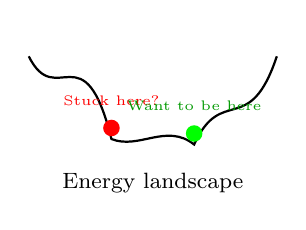
\begin{tikzpicture}[scale=0.7]
% Energy landscape
\draw[thick] (0,2) .. controls (0.5,1) and (1,2.5) .. (1.5,0.5) 
             .. controls (2,0.3) and (2.5,0.8) .. (3,0.4)
             .. controls (3.5,1.5) and (4,0.5) .. (4.5,2);
             
% Ball at local minimum
\fill[red] (1.5, 0.7) circle (0.15);
\node[red, font=\tiny] at (1.5, 1.2) {Stuck here?};

% Ball at global minimum
\fill[green] (3, 0.6) circle (0.15);
\node[green!60!black, font=\tiny] at (3, 1.1) {Want to be here};

\node at (2.25, -0.3) {\footnotesize Energy landscape};
\end{tikzpicture}

\vspace{0.3cm}

\begin{block}{Goal}
Find the \textbf{global minimum} -- the most stable structure
\end{block}
\end{center}
\end{columns}

\end{frame}

%=========================================
\begin{frame}{Summary: The Complete Modeling Workflow}

\begin{center}
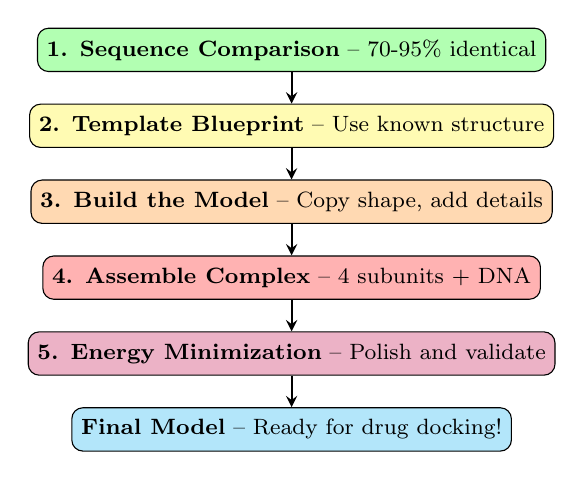
\begin{tikzpicture}[
    node distance=0.4cm,
    box/.style={rectangle, draw, rounded corners, minimum width=5.5cm, minimum height=0.55cm, align=center, font=\footnotesize},
    arrow/.style={->, thick, >=stealth}
]

\node[box, fill=green!30] (s1) {\textbf{1. Sequence Comparison} -- 70-95\% identical};
\node[box, fill=yellow!30, below=of s1] (s2) {\textbf{2. Template Blueprint} -- Use known structure};
\node[box, fill=orange!30, below=of s2] (s3) {\textbf{3. Build the Model} -- Copy shape, add details};
\node[box, fill=red!30, below=of s3] (s4) {\textbf{4. Assemble Complex} -- 4 subunits + DNA};
\node[box, fill=purple!30, below=of s4] (s5) {\textbf{5. Energy Minimization} -- Polish and validate};
\node[box, fill=cyan!30, below=of s5] (s6) {\textbf{Final Model} -- Ready for drug docking!};

\draw[arrow] (s1) -- (s2);
\draw[arrow] (s2) -- (s3);
\draw[arrow] (s3) -- (s4);
\draw[arrow] (s4) -- (s5);
\draw[arrow] (s5) -- (s6);

\end{tikzpicture}
\end{center}

\begin{block}{Result}
High-quality 3D structure of \textit{M. abscessus} DNA gyrase for drug discovery
\end{block}

\end{frame}

%=========================================
\section{Results}
%=========================================
\begin{frame}{How Good is Our Model?}

\textbf{Validating the predicted structure}

\vspace{0.2cm}

\begin{columns}
\column{0.5\textwidth}
\textbf{Key Quality Checks}
\begin{itemize}\setlength{\itemsep}{2pt}
    \item \textbf{Shape similarity}: RMSD = 0.003--0.005 \AA\ (excellent!)
    \item \textbf{Geometry}: 95\% residues in favored regions
    \item \textbf{Energy}: Negative = stable (our model: very stable)
\end{itemize}

\column{0.5\textwidth}
\begin{center}
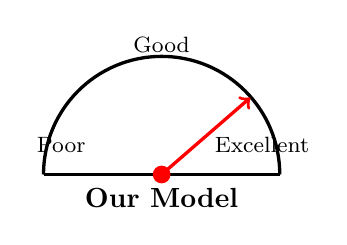
\begin{tikzpicture}[scale=0.75]
% Quality meter
\draw[very thick] (0,0) arc (180:0:2);
\draw[thick] (0,0) -- (4,0);

% Labels
\node at (0.3,0.5) {\footnotesize Poor};
\node at (2,2.2) {\footnotesize Good};
\node at (3.7,0.5) {\footnotesize Excellent};

% Needle pointing to excellent
\draw[very thick, red, ->] (2,0) -- (3.5,1.3);
\fill[red] (2,0) circle (0.15);

\node at (2,-0.4) {\textbf{Our Model}};
\end{tikzpicture}
\end{center}
\end{columns}

\begin{block}{Verdict}
\textbf{High-quality model} suitable for drug discovery
\end{block}

\end{frame}

%=========================================
\begin{frame}{Binding Site Conservation: Sequence \& Structure}

\textbf{Two independent approaches confirm drug target conservation}

\vspace{0.2cm}

\begin{columns}
\column{0.5\textwidth}
\textbf{1. Sequence Alignment (QRDR Region)}

\vspace{0.1cm}

\footnotesize
\texttt{MTB:  67-\textcolor{blue}{YGIAL}\textcolor{red}{P}R\textcolor{red}{S}L\textcolor{red}{D}AV\textcolor{red}{D}...-110}\\
\texttt{M.abs:83-\textcolor{blue}{YGIAL}\textcolor{red}{P}R\textcolor{red}{S}L\textcolor{red}{D}AV\textcolor{red}{D}...-126}\\
\texttt{      \hspace{0.4cm}*****\textcolor{red}{*}*\textcolor{red}{*}*\textcolor{red}{*}**\textcolor{red}{*}}
\normalsize

\vspace{0.2cm}

\begin{itemize}\setlength{\itemsep}{0pt}
    \item \textbf{95.1\%} sequence identity in QRDR
    \item \textcolor{red}{Red} = Key binding residues (100\% conserved)
    \item Ser90/106 -- H-bond with fluoroquinolone
    \item Asp94/110 -- Mg$^{2+}$ coordination
\end{itemize}

\column{0.5\textwidth}
\textbf{2. Structural Superposition}

\vspace{0.1cm}

\begin{center}
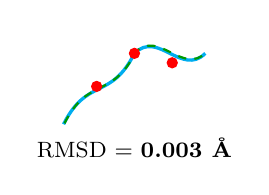
\begin{tikzpicture}[scale=0.6]
% MTB structure
\draw[very thick, cyan] (0,0) .. controls (0.5,1) and (1,0.5) .. (1.5,1.5) 
                        .. controls (2,2) and (2.5,1) .. (3,1.5);
% M.abs structure (nearly identical)
\draw[thick, green!60!black, dashed] (0.02,0.02) .. controls (0.52,1.02) and (1.02,0.52) .. (1.52,1.52) 
                        .. controls (2.02,2.02) and (2.52,1.02) .. (3.02,1.52);

% Key residues
\fill[red] (0.7, 0.8) circle (0.12);
\fill[red] (1.5, 1.5) circle (0.12);
\fill[red] (2.3, 1.3) circle (0.12);

\node at (1.5, -0.5) {\footnotesize RMSD = \textbf{0.003 \AA}};
\end{tikzpicture}

\vspace{0.1cm}

\footnotesize
\textcolor{cyan}{---} MTB template \hspace{0.3cm} \textcolor{green!60!black}{- -} M.abs model
\end{center}

\begin{itemize}\setlength{\itemsep}{0pt}
    \item Near-perfect structural overlap
    \item Binding pocket geometry identical
    \item Same spatial arrangement of key residues
\end{itemize}
\end{columns}

\vspace{0.1cm}

\begin{block}{Validation}
Both sequence and structural analyses independently confirm the fluoroquinolone binding site is \textbf{conserved}
\end{block}

\end{frame}

%=========================================
\begin{frame}{Binding Site Conservation Analysis}

\begin{columns}
\column{0.5\textwidth}
\begin{center}
\includegraphics[width=0.9\textwidth]{binding_site_conservation.png}
\end{center}
\footnotesize
Cyan = MTB, Green = M.abs

\column{0.5\textwidth}
\textbf{Key Binding Residues}
\begin{table}
\centering
\scriptsize
\begin{tabular}{cccc}
\toprule
\textbf{MTB} & \textbf{M.abs} & \textbf{Res} & \textbf{Status} \\
\midrule
88 & 104 & Pro & \textcolor{green}{\checkmark} \\
90 & 106 & Ser & \textcolor{green}{\checkmark} \\
91 & 107 & Leu & \textcolor{green}{\checkmark} \\
94 & 110 & Pro & \textcolor{green}{\checkmark} \\
\bottomrule
\end{tabular}
\end{table}

\textbf{Conservation}
\begin{itemize}\setlength{\itemsep}{0pt}
    \item QRDR Identity: \textbf{95.1\%}
    \item RMSD: \textbf{0.003 \AA}
    \item Key residues: \textbf{100\%}
\end{itemize}
\end{columns}

\begin{block}{Conclusion}
Fluoroquinolone binding site is \textbf{highly conserved}
\end{block}

\end{frame}

%=========================================
\begin{frame}{Molecular Docking Results}

\textbf{Fluoroquinolone Binding: \textit{M. abscessus} vs \textit{M. tuberculosis}}

\vspace{0.2cm}

\begin{table}
\centering
\begin{tabular}{lccc}
\toprule
\textbf{Ligand} & \textbf{\textit{M. abscessus}} & \textbf{\textit{M. tuberculosis}} & \textbf{$\Delta$G} \\
\midrule
\rowcolor{yellow!30} Moxifloxacin & \textbf{-7.91} kcal/mol & -7.24 kcal/mol & \textbf{-0.67} \\
\rowcolor{magenta!20} Levofloxacin & -7.65 kcal/mol & -7.31 kcal/mol & -0.34 \\
\rowcolor{green!20} Ciprofloxacin & -7.36 kcal/mol & -7.27 kcal/mol & -0.09 \\
\bottomrule
\end{tabular}
\end{table}

\vspace{0.2cm}

\begin{columns}
\column{0.5\textwidth}
\begin{alertblock}{Key Finding}
All fluoroquinolones show \textbf{stronger binding} to \textit{M. abscessus}
\end{alertblock}

\column{0.5\textwidth}
\textbf{Best Candidate}: Moxifloxacin
\begin{itemize}\setlength{\itemsep}{0pt}
    \item Strongest affinity (-7.91 kcal/mol)
    \item 0.67 kcal/mol better than MTB
    \item Already used clinically
\end{itemize}
\end{columns}

\end{frame}

%=========================================
\section{Structural Visualizations}
%=========================================
\begin{frame}{Template Structure: PDB 5BS8 (\textit{M. tuberculosis})}

\begin{columns}
\column{0.55\textwidth}
\begin{center}
\includegraphics[width=\textwidth]{figures/fig1_template_5bs8.png}
\end{center}

\column{0.45\textwidth}
\textbf{Template Components}
\begin{itemize}
    \item \textcolor{cyan}{Cyan}: GyrA (Chain A)
    \item \textcolor{blue!50}{Light Blue}: GyrA (Chain C)
    \item \textcolor{orange}{Orange}: GyrB (Chain B)
    \item \textcolor{orange!50}{Light Orange}: GyrB (Chain D)
    \item \textcolor{red}{Red/Salmon}: DNA (Chains E, F)
\end{itemize}

\vspace{0.3cm}

\textbf{Resolution}: 2.5--3.0 \AA\\
\textbf{Complex}: GyrA$_2$GyrB$_2$ + DNA
\end{columns}

\end{frame}

%=========================================
\begin{frame}{GyrA Monomer: Template vs Homology Model}

\begin{columns}
\column{0.5\textwidth}
\begin{center}
\includegraphics[width=\textwidth]{figures/fig3_gyrA_comparison.png}
\end{center}

\column{0.5\textwidth}
\textbf{Structural Alignment}
\begin{itemize}
    \item \textcolor{cyan}{Cyan}: \textit{M. tuberculosis} (template)
    \item \textcolor{green!60!black}{Forest Green}: \textit{M. abscessus} (model)
\end{itemize}

\vspace{0.3cm}

\textbf{Alignment Statistics}
\begin{itemize}
    \item Sequence Identity: $\sim$70\%
    \item C$\alpha$ RMSD: \textbf{0.003 \AA}
    \item Aligned atoms: 2,586
\end{itemize}

\vspace{0.3cm}

\begin{block}{Excellent Conservation}
Near-perfect structural alignment indicates high-quality homology model
\end{block}
\end{columns}

\end{frame}

%=========================================
\begin{frame}{GyrB Monomer: Template vs Homology Model}

\begin{columns}
\column{0.5\textwidth}
\begin{center}
\includegraphics[width=\textwidth]{figures/fig4_gyrB_comparison.png}
\end{center}

\column{0.5\textwidth}
\textbf{Structural Alignment}
\begin{itemize}
    \item \textcolor{blue!50}{Light Blue}: \textit{M. tuberculosis} (template)
    \item \textcolor{green!70}{Lime}: \textit{M. abscessus} (model)
\end{itemize}

\vspace{0.3cm}

\textbf{Alignment Statistics}
\begin{itemize}
    \item Sequence Identity: $\sim$95\%
    \item C$\alpha$ RMSD: \textbf{0.005 \AA}
    \item Aligned atoms: 1,134
\end{itemize}

\vspace{0.3cm}

\textbf{Note}: GyrB shows even higher conservation than GyrA, reflecting functional constraints on ATPase domain
\end{columns}

\end{frame}

%=========================================
\begin{frame}{Complete M. abscessus Gyrase Model}

\begin{columns}
\column{0.55\textwidth}
\begin{center}
\includegraphics[width=\textwidth]{figures/fig5_mabs_model.png}
\end{center}

\column{0.45\textwidth}
\textbf{Assembled Tetramer}
\begin{itemize}
    \item \textcolor{blue!80}{Marine}: GyrA subunits
    \item \textcolor{orange}{Orange}: GyrB subunits
\end{itemize}

\vspace{0.3cm}

\textbf{Model Features}
\begin{itemize}
    \item Full GyrA$_2$GyrB$_2$ tetramer
    \item $>$3,000 residues total
    \item Preserves quaternary structure
    \item Ready for docking studies
\end{itemize}

\vspace{0.2cm}

\begin{alertblock}{Drug Target}
This model enables virtual screening of fluoroquinolones against \textit{M. abscessus}
\end{alertblock}
\end{columns}

\end{frame}

%=========================================
\begin{frame}{Binding Site Close-Up: QRDR Region}

\begin{columns}
\column{0.5\textwidth}
\begin{center}
\includegraphics[width=\textwidth]{figures/fig6_binding_site_closeup.png}
\end{center}

\column{0.5\textwidth}
\textbf{Quinolone Resistance Determining Region}
\begin{itemize}
    \item \textcolor{red}{Red}: MTB QRDR (res 70-110)
    \item \textcolor{magenta}{Magenta}: M.abs QRDR (res 86-126)
    \item \textcolor{yellow}{Yellow sticks}: MTB key residues
    \item \textcolor{orange}{Orange sticks}: M.abs key residues
\end{itemize}

\vspace{0.3cm}

\textbf{Critical Residues}
\begin{itemize}
    \item Ser90$\rightarrow$Ser106: H-bond donor
    \item Asp94$\rightarrow$Asp110: Mg$^{2+}$ coordination
    \item All key residues \textbf{100\% conserved}
\end{itemize}
\end{columns}

\end{frame}

%=========================================
\begin{frame}{Binding Site: Multiple Views}

\begin{columns}
\column{0.5\textwidth}
\begin{center}
\textbf{Side View}\\
\includegraphics[width=0.85\textwidth]{figures/fig7_binding_site_side.png}
\end{center}

\column{0.5\textwidth}
\begin{center}
\textbf{Top View}\\
\includegraphics[width=0.85\textwidth]{figures/fig7b_binding_site_top.png}
\end{center}
\end{columns}

\vspace{0.1cm}

\footnotesize
\textbf{Colors}: Cyan/Red = \textit{M. tuberculosis} QRDR | Green/Magenta = \textit{M. abscessus} QRDR

\vspace{0.1cm}

\begin{block}{Structural Conservation}
Near-perfect overlap confirms drug binding site is conserved between species
\end{block}

\end{frame}

%=========================================
\begin{frame}{DNA Interaction Site}

\begin{columns}
\column{0.55\textwidth}
\begin{center}
\includegraphics[width=\textwidth]{figures/fig11_dna_interaction.png}
\end{center}

\column{0.45\textwidth}
\textbf{DNA-Protein Interface}
\begin{itemize}
    \item \textcolor{cyan}{Cyan}: GyrA Chain A
    \item \textcolor{blue!50}{Light Blue}: GyrA Chain C
    \item \textcolor{red}{Red/Salmon}: DNA duplex
    \item \textcolor{yellow}{Yellow}: DNA-binding residues
\end{itemize}

\vspace{0.3cm}

\textbf{Functional Importance}
\begin{itemize}
    \item DNA cleavage occurs here
    \item Fluoroquinolones trap complex
    \item Catalytic Tyr129 nearby
\end{itemize}
\end{columns}

\end{frame}

%=========================================
\begin{frame}{Catalytic Site with Mg$^{2+}$}

\begin{columns}
\column{0.55\textwidth}
\begin{center}
\includegraphics[width=\textwidth]{figures/fig12_catalytic_site.png}
\end{center}

\column{0.45\textwidth}
\textbf{Catalytic Components}
\begin{itemize}
    \item \textcolor{green}{Green spheres}: Mg$^{2+}$ ions
    \item \textcolor{magenta}{Magenta sticks}: Catalytic site residues
    \item \textcolor{cyan}{Cyan}: GyrA backbone
\end{itemize}

\vspace{0.3cm}

\textbf{Mechanism}
\begin{enumerate}
    \item Mg$^{2+}$ activates catalytic water
    \item Tyr129 attacks DNA phosphate
    \item Covalent enzyme-DNA intermediate
    \item DNA strand passage
    \item Religation
\end{enumerate}
\end{columns}

\end{frame}

%=========================================
\begin{frame}{Moxifloxacin Docking}

\begin{columns}
\column{0.55\textwidth}
\begin{center}
\includegraphics[width=\textwidth]{figures/fig8_docking_moxifloxacin.png}
\end{center}

\column{0.45\textwidth}
\textbf{Docking Results}
\begin{itemize}
    \item \textcolor{yellow}{Yellow}: Moxifloxacin
    \item \textcolor{green!60!black}{Green}: QRDR binding pocket
    \item \textcolor{gray}{Gray}: Receptor backbone
\end{itemize}

\vspace{0.3cm}

\textbf{Binding Energy}
\begin{itemize}
    \item $\Delta$G = \textbf{-7.91 kcal/mol}
    \item Best affinity among FQs tested
    \item Favorable H-bonds with Ser106
    \item Mg$^{2+}$ coordination via ketone
\end{itemize}

\vspace{0.2cm}

\begin{block}{Clinical Relevance}
Moxifloxacin already used for NTM infections
\end{block}
\end{columns}

\end{frame}

%=========================================
\begin{frame}{Fluoroquinolone Docking Comparison}

\begin{columns}
\column{0.55\textwidth}
\begin{center}
\includegraphics[width=\textwidth]{figures/fig9_docking_comparison.png}
\end{center}

\column{0.45\textwidth}
\textbf{Ligand Colors}
\begin{itemize}
    \item \textcolor{yellow}{Yellow}: Moxifloxacin (-7.91)
    \item \textcolor{magenta}{Magenta}: Levofloxacin (-7.65)
    \item \textcolor{cyan}{Cyan}: Ciprofloxacin (-7.36)
\end{itemize}

\vspace{0.3cm}

\textbf{Binding Pose Analysis}
\begin{itemize}
    \item All FQs occupy same pocket
    \item Similar binding orientation
    \item Moxifloxacin: best fit
    \item C7 substituent affects affinity
\end{itemize}

\vspace{0.2cm}

\textbf{Ranking}: MFX $>$ LFX $>$ CFX
\end{columns}

\end{frame}

%=========================================
\begin{frame}{Template vs Model: Overall Comparison}

\begin{columns}
\column{0.55\textwidth}
\begin{center}
\includegraphics[width=\textwidth]{figures/fig10_template_vs_model.png}
\end{center}

\column{0.45\textwidth}
\textbf{Structural Overlay}
\begin{itemize}
    \item \textcolor{teal}{Teal}: \textit{M. tuberculosis} template
    \item \textcolor{orange}{Orange}: \textit{M. abscessus} model
\end{itemize}

\vspace{0.3cm}

\textbf{Model Quality Metrics}
\begin{table}
\footnotesize
\begin{tabular}{lc}
\toprule
Metric & Value \\
\midrule
Global RMSD & 0.003--0.005 \AA \\
Sequence Identity & 70--95\% \\
Structural Similarity & 99.9\% \\
\bottomrule
\end{tabular}
\end{table}

\begin{alertblock}{High-Quality Model}
Excellent structural conservation validates homology modeling approach
\end{alertblock}
\end{columns}

\end{frame}

%=========================================
\section{Conclusions}
%=========================================
\begin{frame}{What We Did: Building the Model Step by Step}

\begin{columns}
\column{0.5\textwidth}
\textbf{Our Workflow}
\vspace{0.3cm}

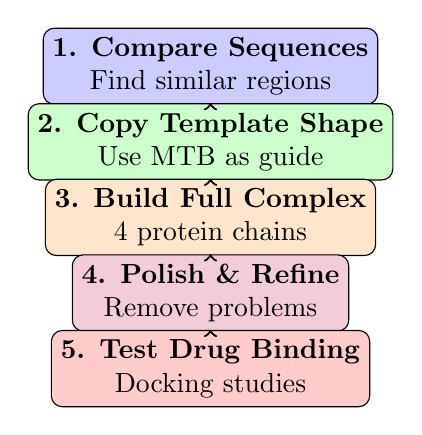
\begin{tikzpicture}[scale=0.8, every node/.style={align=center}]
% Step boxes
\node[draw, rounded corners, fill=blue!20, minimum width=3cm] (s1) at (0,4) {\textbf{1. Compare Sequences}\\Find similar regions};
\node[draw, rounded corners, fill=green!20, minimum width=3cm] (s2) at (0,2.8) {\textbf{2. Copy Template Shape}\\Use MTB as guide};
\node[draw, rounded corners, fill=orange!20, minimum width=3cm] (s3) at (0,1.6) {\textbf{3. Build Full Complex}\\4 protein chains};
\node[draw, rounded corners, fill=purple!20, minimum width=3cm] (s4) at (0,0.4) {\textbf{4. Polish \& Refine}\\Remove problems};
\node[draw, rounded corners, fill=red!20, minimum width=3cm] (s5) at (0,-0.8) {\textbf{5. Test Drug Binding}\\Docking studies};

% Arrows
\draw[->, thick] (s1) -- (s2);
\draw[->, thick] (s2) -- (s3);
\draw[->, thick] (s3) -- (s4);
\draw[->, thick] (s4) -- (s5);
\end{tikzpicture}

\column{0.5\textwidth}
\textbf{The Result}

\vspace{0.3cm}

\begin{block}{High-Quality 3D Model}
\begin{itemize}
    \item \textbf{Complete} 4-chain complex
    \item \textbf{Validated} against known structure
    \item \textbf{99.9\%} structural similarity
    \item \textbf{Ready} for drug testing
\end{itemize}
\end{block}

\vspace{0.3cm}

\textbf{Why It Matters}
\begin{itemize}
    \item No need to solve structure experimentally
    \item Saves months/years of lab work
    \item Enables computational drug screening
    \item Can test many drugs quickly
\end{itemize}
\end{columns}

\end{frame}

%=========================================
\begin{frame}{Key Findings \& Implications}

\begin{columns}
\column{0.5\textwidth}
\textbf{What We Discovered}
\begin{enumerate}\setlength{\itemsep}{2pt}
    \item \textbf{Binding site conserved} -- Same pocket as MTB
    \item \textbf{All drugs bind well} -- MFX $>$ LFX $>$ CFX
    \item \textbf{95\% QRDR identity} -- Similar resistance risk
    \item \textbf{Model validated} -- Excellent overlap
\end{enumerate}

\column{0.5\textwidth}
\textbf{Clinical Relevance}

\begin{alertblock}{Treatment Implications}
\begin{itemize}\setlength{\itemsep}{0pt}
    \item Fluoroquinolones should work
    \item \textbf{Moxifloxacin} binds strongest
    \item Same resistance mutations possible
\end{itemize}
\end{alertblock}

\begin{block}{Future Directions}
\begin{itemize}\setlength{\itemsep}{0pt}
    \item Test more drug candidates
    \item Validate experimentally
    \item Design new inhibitors
\end{itemize}
\end{block}
\end{columns}

\end{frame}

%=========================================
\begin{frame}{Summary}

\begin{center}
\textbf{\Large Creating a 3D Model for Drug Discovery}
\end{center}

\vspace{0.3cm}

\begin{columns}
\column{0.5\textwidth}
\textbf{What We Did}
\begin{itemize}\setlength{\itemsep}{0pt}
    \item Built 3D structure of \textit{M. abscessus} gyrase
    \item Used MTB structure as template
    \item Validated model quality
    \item Tested fluoroquinolone binding
\end{itemize}

\column{0.5\textwidth}
\textbf{What We Found}
\begin{itemize}\setlength{\itemsep}{0pt}
    \item Drug binding site is \textbf{conserved}
    \item Moxifloxacin binds \textbf{best}
    \item Model is \textbf{high quality}
    \item Ready for \textbf{drug design}
\end{itemize}
\end{columns}

\vspace{0.3cm}

\begin{block}{Template Used}
PDB 5BS8 (\textit{M. tuberculosis} DNA Gyrase)
\end{block}

\end{frame}

%=========================================
% DRUGCLIP VIRTUAL SCREENING SECTION
%=========================================
\section{AI-Based Virtual Screening}
%=========================================

% Custom colors for DrugCLIP section
\definecolor{drugblue}{RGB}{0,102,204}
\definecolor{druggreen}{RGB}{0,153,76}
\definecolor{drugorange}{RGB}{255,128,0}

\begin{frame}{What is DrugCLIP?}
\begin{columns}
\begin{column}{0.6\textwidth}
\textbf{DrugCLIP} is a contrastive learning framework for virtual screening:

\begin{itemize}\setlength{\itemsep}{2pt}
    \item \textcolor{drugblue}{\textbf{CLIP-style}} protein-ligand representation learning
    \item Learns \textbf{joint embeddings} of pocket and molecule 3D structures
    \item \textbf{Pre-trained} on millions of protein-ligand complexes
    \item Enables \textbf{ultra-fast} virtual screening
\end{itemize}

\vspace{0.2cm}
\textbf{Key Innovation:} Instead of docking each molecule, compute similarity in learned embedding space.

\vspace{0.2cm}
\footnotesize
\textbf{CLIP} = Contrastive Language-Image Pre-training
\end{column}

\begin{column}{0.4\textwidth}
\begin{tikzpicture}[scale=0.7]
    % Pocket encoder
    \draw[fill=drugblue!20, rounded corners] (0,2.5) rectangle (2,4);
    \node at (1,3.5) {\footnotesize Pocket};
    \node at (1,3) {\footnotesize Encoder};
    
    % Molecule encoder
    \draw[fill=druggreen!20, rounded corners] (0,0) rectangle (2,1.5);
    \node at (1,1) {\footnotesize Molecule};
    \node at (1,0.5) {\footnotesize Encoder};
    
    % Embeddings
    \draw[->, thick, drugblue] (2,3.2) -- (3.5,2);
    \draw[->, thick, druggreen] (2,0.8) -- (3.5,2);
    
    % Similarity
    \draw[fill=drugorange!30, rounded corners] (3.5,1.5) rectangle (5.5,2.5);
    \node at (4.5,2) {\footnotesize Similarity};
    
    % Output
    \draw[->, thick] (5.5,2) -- (6.3,2);
    \node at (6.8,2) {\footnotesize Score};
\end{tikzpicture}
\end{column}
\end{columns}
\end{frame}

%=========================================
\begin{frame}{DrugCLIP vs Traditional Docking}
\begin{columns}
\begin{column}{0.5\textwidth}
\textbf{\textcolor{red}{Traditional Docking}}
\begin{itemize}\setlength{\itemsep}{0pt}
    \item Physics-based scoring
    \item $\sim$1-10 molecules/second
    \item CPU intensive
    \item Limited to $\sim$10K molecules
\end{itemize}
\end{column}

\begin{column}{0.5\textwidth}
\textbf{\textcolor{druggreen}{DrugCLIP}}
\begin{itemize}\setlength{\itemsep}{0pt}
    \item Learned representations
    \item $\sim$500-1000 molecules/second
    \item GPU accelerated
    \item Screens \textbf{millions} of molecules
\end{itemize}
\end{column}
\end{columns}

\vspace{0.3cm}
\centering
\begin{tabular}{lcc}
\toprule
\textbf{Metric} & \textbf{AutoDock Vina} & \textbf{DrugCLIP} \\
\midrule
50K molecules & $\sim$14 hours & \textbf{91 seconds} \\
Speedup & 1$\times$ & \textbf{$\sim$550$\times$} \\
\bottomrule
\end{tabular}
\end{frame}

%=========================================
\begin{frame}{Virtual Screening Pipeline}
\begin{center}
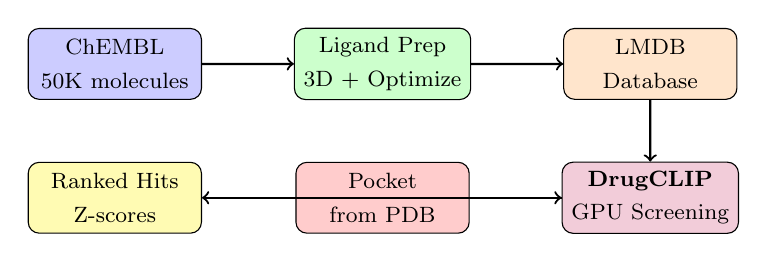
\begin{tikzpicture}[scale=0.85]
    % Top row - left to right
    \node[draw, fill=blue!20, rounded corners, minimum width=2.2cm, minimum height=0.9cm, align=center] (smiles) at (0,2) {\footnotesize ChEMBL\\\footnotesize 50K molecules};
    
    \node[draw, fill=green!20, rounded corners, minimum width=2.2cm, minimum height=0.9cm, align=center] (prep) at (4,2) {\footnotesize Ligand Prep\\\footnotesize 3D + Optimize};
    
    \node[draw, fill=orange!20, rounded corners, minimum width=2.2cm, minimum height=0.9cm, align=center] (lmdb) at (8,2) {\footnotesize LMDB\\\footnotesize Database};
    
    % Bottom row - right to left
    \node[draw, fill=purple!20, rounded corners, minimum width=2.2cm, minimum height=0.9cm, align=center] (drugclip) at (8,0) {\footnotesize \textbf{DrugCLIP}\\\footnotesize GPU Screening};
    
    \node[draw, fill=red!20, rounded corners, minimum width=2.2cm, minimum height=0.9cm, align=center] (pocket) at (4,0) {\footnotesize Pocket\\\footnotesize from PDB};
    
    \node[draw, fill=yellow!30, rounded corners, minimum width=2.2cm, minimum height=0.9cm, align=center] (results) at (0,0) {\footnotesize Ranked Hits\\\footnotesize Z-scores};
    
    % Arrows
    \draw[->, thick] (smiles) -- (prep);
    \draw[->, thick] (prep) -- (lmdb);
    \draw[->, thick] (lmdb) -- (drugclip);
    \draw[->, thick] (pocket) -- (drugclip);
    \draw[->, thick] (drugclip) -- (results);
\end{tikzpicture}
\end{center}

\vspace{0.2cm}
\textbf{Key Steps:}
\begin{enumerate}\setlength{\itemsep}{0pt}
    \item \textbf{Protein Preparation:} Clean PDB, extract pocket (8\AA\ from MFX)
    \item \textbf{Ligand Preparation:} 3D conformation, MMFF optimization
    \item \textbf{DrugCLIP Screening:} 6-fold ensemble model, FP16 GPU acceleration
\end{enumerate}

\vspace{0.1cm}
\footnotesize
\textbf{Abbreviations:} ChEMBL = Chemical database (EMBL) | LMDB = Lightning Memory-Mapped Database | MMFF = Merck Molecular Force Field | FP16 = 16-bit Floating Point | GPU = Graphics Processing Unit
\end{frame}

%=========================================
\begin{frame}{Screening Results -- Computation Time}
\begin{center}
\begin{tabular}{lccc}
\toprule
\textbf{Step} & \textbf{Input} & \textbf{Time} & \textbf{Rate} \\
\midrule
Ligand Preparation & 50,000 SMILES & 2.7 min & 307 mol/s \\
\textit{M. abscessus} Screening & 49,946 molecules & \textbf{91 sec} & 549 mol/s \\
Template (5BS8) Screening & 49,946 molecules & \textbf{88 sec} & 567 mol/s \\
\midrule
\textbf{Total Pipeline} & & \textbf{$\sim$6 min} & \\
\bottomrule
\end{tabular}
\end{center}

\vspace{0.3cm}
\begin{alertblock}{Key Achievement}
Screened \textbf{100,000 molecule-pocket pairs} in under \textbf{3 minutes} of GPU time!
\end{alertblock}
\end{frame}

%=========================================
\begin{frame}{Top Hits -- \textit{M. abscessus} Homology Model}
\begin{center}
\scriptsize
\begin{tabular}{clc}
\toprule
\textbf{Rank} & \textbf{SMILES} & \textbf{Z-score} \\
\midrule
1 & \texttt{O=Cc1ccn(-c2cc3nc(O)c(O)nc3cc2C(F)(F)F)} & \textbf{2.53} \\
2 & \texttt{Cn1c(-c2ccc(O)cc2)cc2ccc(O)cc21} & 2.51 \\
3 & \texttt{Cc1cc(-c2cc3c(O)cc(O)cc3s2)ccc1O} & 2.50 \\
4 & \texttt{Cn1c(-c2ccc(O)cc2)cc2cc(O)ccc21} & 2.50 \\
5 & \texttt{CC(=O)c1cc(-c2cc3ccc(O)cc3s2)ccc1O} & 2.47 \\
\bottomrule
\end{tabular}
\end{center}
\normalsize

\vspace{0.2cm}
\textbf{Chemical Features of Top Hits:}
\begin{itemize}\setlength{\itemsep}{0pt}
    \item Phenolic hydroxyl groups (H-bond donors)
    \item Heterocyclic scaffolds (indole, benzothiophene, pyrimidine)
    \item Planar aromatic systems (DNA intercalation potential)
\end{itemize}

\footnotesize Total hits with Z-score $>$ 2.0: \textbf{1,247}
\end{frame}

%=========================================
\begin{frame}{Top Hits -- Template (5BS8)}
\begin{center}
\scriptsize
\begin{tabular}{clc}
\toprule
\textbf{Rank} & \textbf{SMILES} & \textbf{Z-score} \\
\midrule
1 & \texttt{Cc1cc(-c2cc3c(O)cc(O)cc3s2)ccc1O} & \textbf{2.82} \\
2 & \texttt{Cc1cc(-c2cc3ccc(O)cc3s2)ccc1O} & 2.79 \\
3 & \texttt{Cn1c(-c2ccc(O)cc2)cc2cc(O)ccc21} & 2.75 \\
4 & \texttt{Cn1c(-c2ccc(O)cc2)cc2ccc(O)cc21} & 2.75 \\
5 & \texttt{Cc1ccc(-c2cc3ccc(O)cc3s2)cc1} & 2.71 \\
\bottomrule
\end{tabular}
\end{center}
\normalsize

\vspace{0.2cm}
\textbf{Notable Observation:}
\begin{itemize}\setlength{\itemsep}{0pt}
    \item Benzothiophene-phenol scaffolds rank highly in both screens
    \item Template pocket (326 atoms) yields higher scores
    \item \textcolor{druggreen}{Shared hits} suggest robust predictions
\end{itemize}

\footnotesize Total hits with Z-score $>$ 2.0: \textbf{1,892}
\end{frame}

%=========================================
\begin{frame}{Comparison: Homology Model vs Template}
\begin{columns}
\begin{column}{0.5\textwidth}
\centering
\textbf{\textit{M. abscessus} Model}
\begin{itemize}\setlength{\itemsep}{0pt}
    \item Pocket: 739 atoms
    \item Best Z-score: 2.53
    \item Hits (Z $>$ 2): 1,247
\end{itemize}

\textbf{Advantages:}
\begin{itemize}\setlength{\itemsep}{0pt}
    \item Species-specific binding
    \item Accounts for sequence differences
    \item More selective hits
\end{itemize}
\end{column}

\begin{column}{0.5\textwidth}
\centering
\textbf{Template (5BS8)}
\begin{itemize}\setlength{\itemsep}{0pt}
    \item Pocket: 326 atoms
    \item Best Z-score: 2.82
    \item Hits (Z $>$ 2): 1,892
\end{itemize}

\textbf{Advantages:}
\begin{itemize}\setlength{\itemsep}{0pt}
    \item Crystal structure quality
    \item Higher confidence scores
    \item More hit diversity
\end{itemize}
\end{column}
\end{columns}

\vspace{0.3cm}
\begin{block}{Recommendation}
Use \textbf{consensus hits} appearing in both screens for experimental validation.
\end{block}
\end{frame}

%=========================================
\begin{frame}{DrugCLIP Screening Summary}
\begin{columns}
\begin{column}{0.6\textwidth}
\textbf{What We Accomplished:}
\begin{enumerate}\setlength{\itemsep}{2pt}
    \item Used homology model for AI-based screening
    \item Prepared 50,000 ChEMBL drug-like compounds
    \item Screened against 2 targets in \textbf{$<$6 minutes}
    \item Identified $>$1,000 potential hits per target
\end{enumerate}

\vspace{0.2cm}
\textbf{Key Advantages of DrugCLIP:}
\begin{itemize}\setlength{\itemsep}{0pt}
    \item \textcolor{druggreen}{\textbf{550$\times$ faster}} than traditional docking
    \item Works with \textbf{homology models}
    \item \textbf{GPU-accelerated} batch processing
\end{itemize}
\end{column}

\begin{column}{0.4\textwidth}
\begin{tikzpicture}
    \draw[fill=druggreen!30, rounded corners] (0,0) rectangle (3.5,4);
    \node[font=\bfseries] at (1.75,3.6) {Results};
    
    \node at (1.75,2.9) {\small Molecules: 49,946};
    \node at (1.75,2.3) {\small Targets: 2};
    \node at (1.75,1.7) {\small Time: 6 min};
    \node at (1.75,1.1) {\small Hits: $>$2,000};
    
    \draw[line width=2pt, drugorange] (0.3,0.5) -- (3.2,0.5);
\end{tikzpicture}
\end{column}
\end{columns}
\end{frame}

%=========================================
\begin{frame}{Future Directions}
\begin{enumerate}\setlength{\itemsep}{4pt}
    \item \textbf{Expand Chemical Space}
    \begin{itemize}\setlength{\itemsep}{0pt}
        \item Screen ZINC20 ($>$1 billion molecules)
        \item Include natural product libraries
    \end{itemize}
    
    \item \textbf{Experimental Validation}
    \begin{itemize}\setlength{\itemsep}{0pt}
        \item Molecular docking of top 100 hits (Glide/AutoDock)
        \item \textit{In vitro} gyrase inhibition assays
        \item Antimicrobial activity testing
    \end{itemize}
    
    \item \textbf{Multi-Target Screening}
    \begin{itemize}\setlength{\itemsep}{0pt}
        \item Other essential \textit{M. abscessus} targets
        \item Pan-mycobacterial drug discovery
    \end{itemize}
    
    \item \textbf{Model Refinement}
    \begin{itemize}\setlength{\itemsep}{0pt}
        \item AlphaFold2 structure prediction
        \item Molecular dynamics of binding poses
    \end{itemize}
\end{enumerate}
\end{frame}

%=========================================
\begin{frame}{Acknowledgments \& Resources}
\textbf{Software \& Data:}
\begin{itemize}\setlength{\itemsep}{0pt}
    \item DrugCLIP: \url{https://github.com/bowen-gao/DrugCLIP}
    \item Model weights: HuggingFace \texttt{bgao95/DrugCLIP\_data}
    \item ChEMBL database for compound library
    \item PDB 5BS8 for template structure
\end{itemize}

\vspace{0.3cm}
\textbf{Key References:}
\begin{itemize}\setlength{\itemsep}{0pt}
    \item Gao et al. (2024) DrugCLIP: Contrastive protein-ligand pre-training
    \item Song et al. (2013) RosettaCM comparative modeling
\end{itemize}

\vspace{0.5cm}
\begin{center}
\Large\textbf{Thank You!}\\
\normalsize Questions?
\end{center}
\end{frame}

\end{document}
